\documentclass{beamer}

\mode<presentation>
{
  \usetheme{default}      % or try Darmstadt, Madrid, Warsaw, ...
  \usecolortheme{default} % or try albatross, beaver, crane, ...
  \usefonttheme{default}  % or try serif, structurebold, ...
  \setbeamertemplate{navigation symbols}{}
  \setbeamertemplate{caption}[numbered]
} 

\usepackage[french]{babel}
\usepackage[utf8x]{inputenc}
\usepackage{fancyvrb}
\usepackage{graphicx}

\author{David Wong
  \and Jacques Monin
  \and Hugo Bonnin}

\title{Implémentation et Analyse d'une White-box du DES}

\institute{Université de Bordeaux}

\date{2014}

\begin{document}

\begin{frame}
  \titlepage
\end{frame}


\begin{frame}{Plan}
  \tableofcontents
\end{frame}

\section{A quoi ça sert ?}

\begin{frame}{A quoi ça sert ?}

\begin{figure}[h]
    \centering
    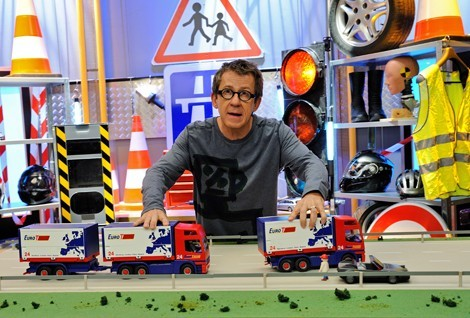
\includegraphics[scale=0.6]{./images/kezako.jpg}
  \end{figure}

\end{frame}

\subsection{Man In The Middle}

\begin{frame}{Base de la cryptographie}

  \begin{figure}[h]
    \centering
    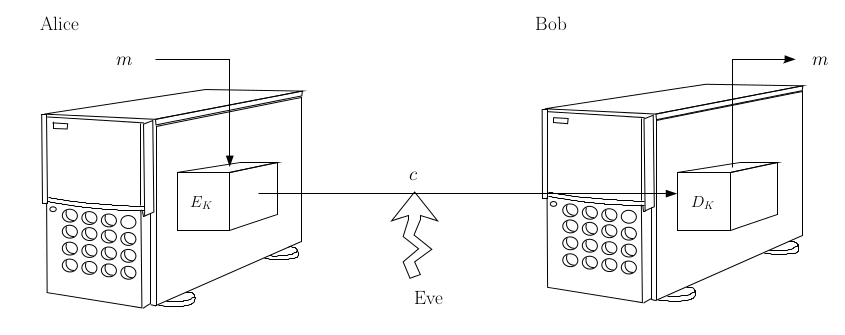
\includegraphics[scale=0.50]{./images/alice_bob.png}
  \end{figure}

\end{frame}

\subsection{Man At The End}

\begin{frame}[fragile]{Man At The End}

\begin{Verbatim}[samepage=true]
                 .-----------------. 
                 |    ATTAQUANT    |
                 |  .-----------.  |  
                 |  |           |  |  
                 |  | PROGRAMME |  | 
                 |  |           |  | 
                 |  '-----------'  |
                 |                 |
                 '-----------------'
\end{Verbatim}
\end{frame}

\subsection{Exemples}

\begin{frame}{Exemples}

 \begin{figure}[h]
    \centering
    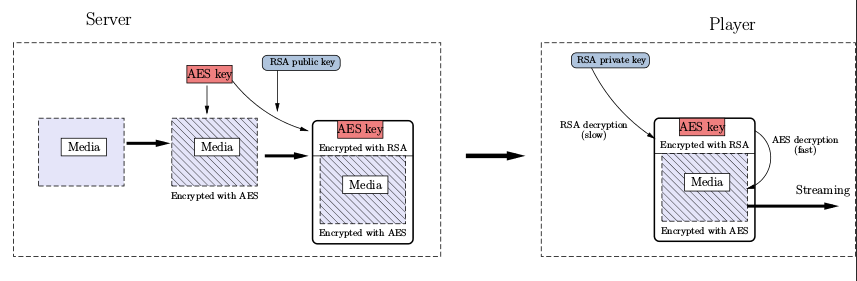
\includegraphics[scale=0.50]{./images/drms.png}
  \end{figure}

\end{frame}

\section{Whitebox}

\subsection{Définition}

\begin{frame}{Définition}

  \begin{figure}[h]
    \centering
    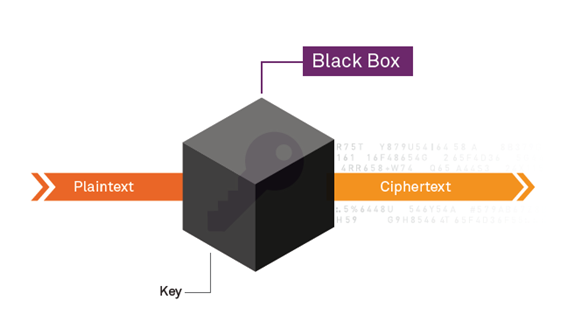
\includegraphics[scale=0.30]{./images/blackbox.png}
  \end{figure}

  \begin{figure}[h]
    \centering
    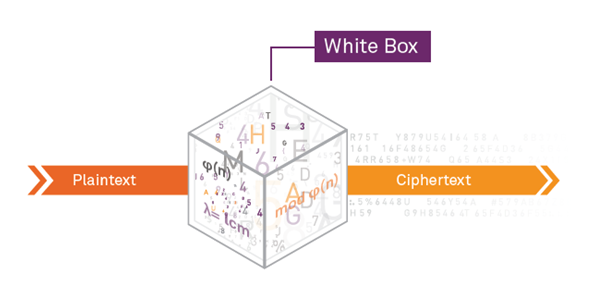
\includegraphics[scale=0.30]{./images/whitebox.png}
  \end{figure}

\end{frame}

\subsection{DES}
\begin{frame}{Algorithme DES}
  \begin{itemize}
  \item Le but est de transformer toutes ces opérations
    \begin{figure}[h]
      \centering
      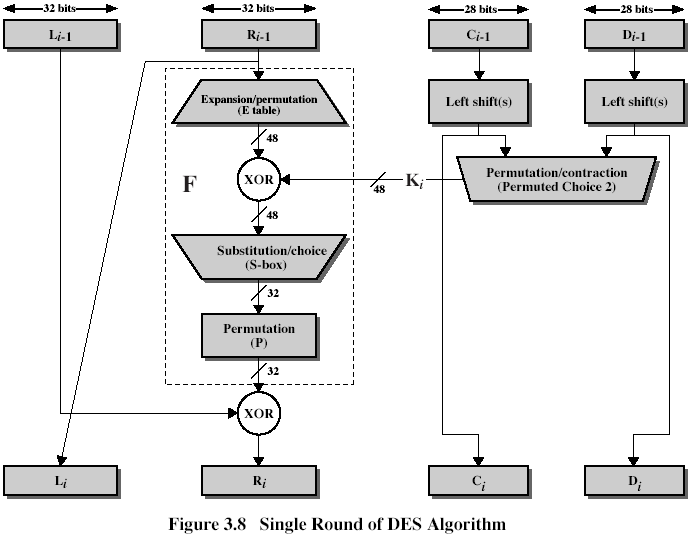
\includegraphics[scale=0.45]{./images/des_slides.png}
      \label{fig:DES-round}
    \end{figure}
  \end{itemize}

\end{frame}

\subsection{Github}
\begin{frame}{Github}
  \begin{itemize}
  \item DES : www.github.com/mimoo/DES
  \item WHITEBOX-DES : www.github.com/mimoo/whiteboxDES
  \end{itemize}

  \begin{figure}[h]
    \centering
    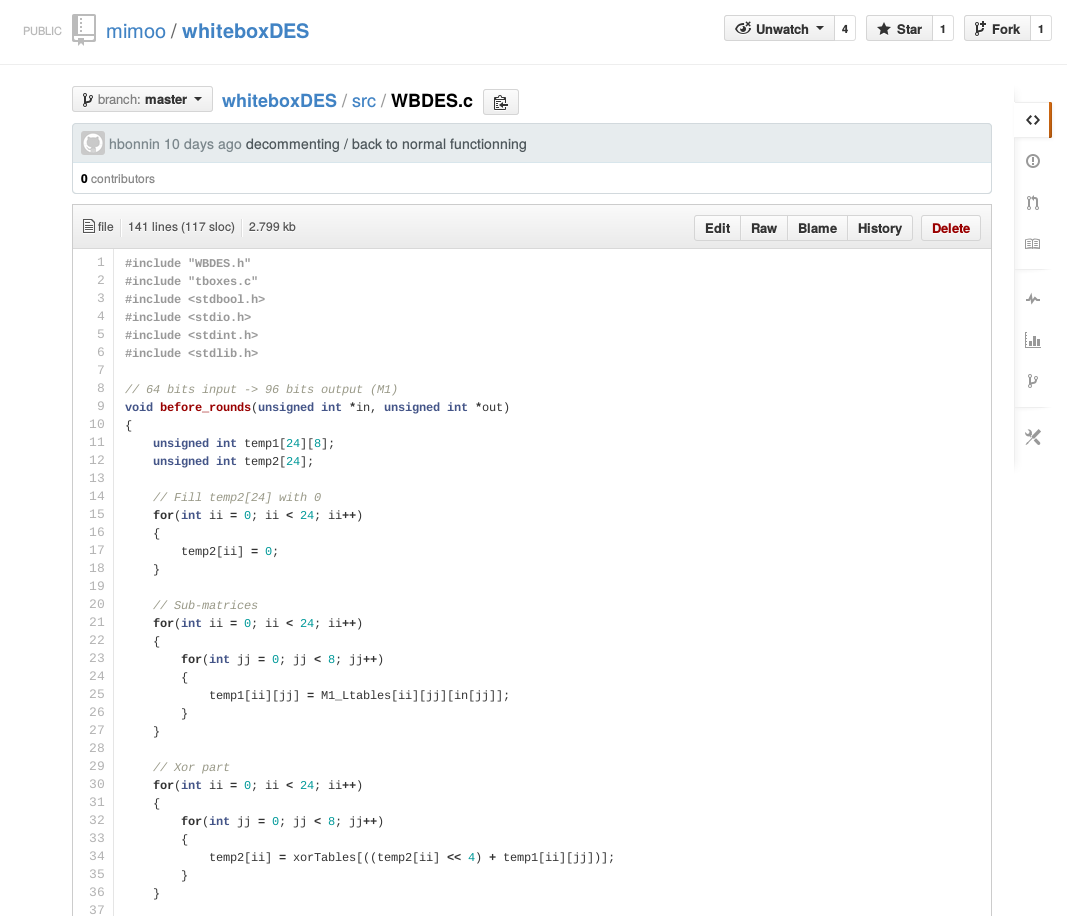
\includegraphics[scale=0.30]{./images/github.png}
  \end{figure}
\end{frame}

\section{Concepts}

\subsection{Partial Evaluation}
\begin{frame}{Partial evaluation}
\begin{itemize}
\item Regrouper le XOR entre le bloc et la clé avec l'opération de substitution.
\item On peut ensuite pré-calculer toutes les sorties possibles de cette opération.
\item Les tables créées sont les seules du programme à être modifiées lorsqu'une nouvelle clé est utilisée.
\end{itemize}
\end{frame}


\subsection{Tabularization}

\begin{frame}[fragile]{Tabularization}
\begin{figure}[h]
\centering
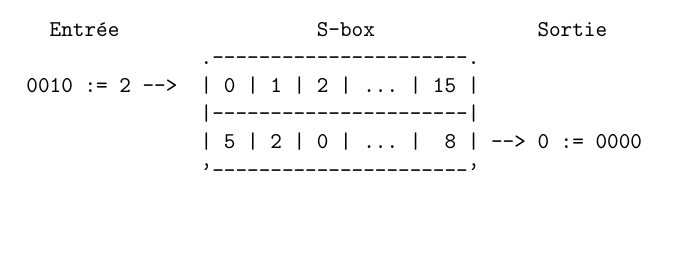
\includegraphics[scale=0.60]{images/tabu.png}
\caption{Tabularisation}
\label{fig:keygen}
\end{figure}
\end{frame}

\begin{frame}{Transformation}
\begin{figure}[h]
\centering
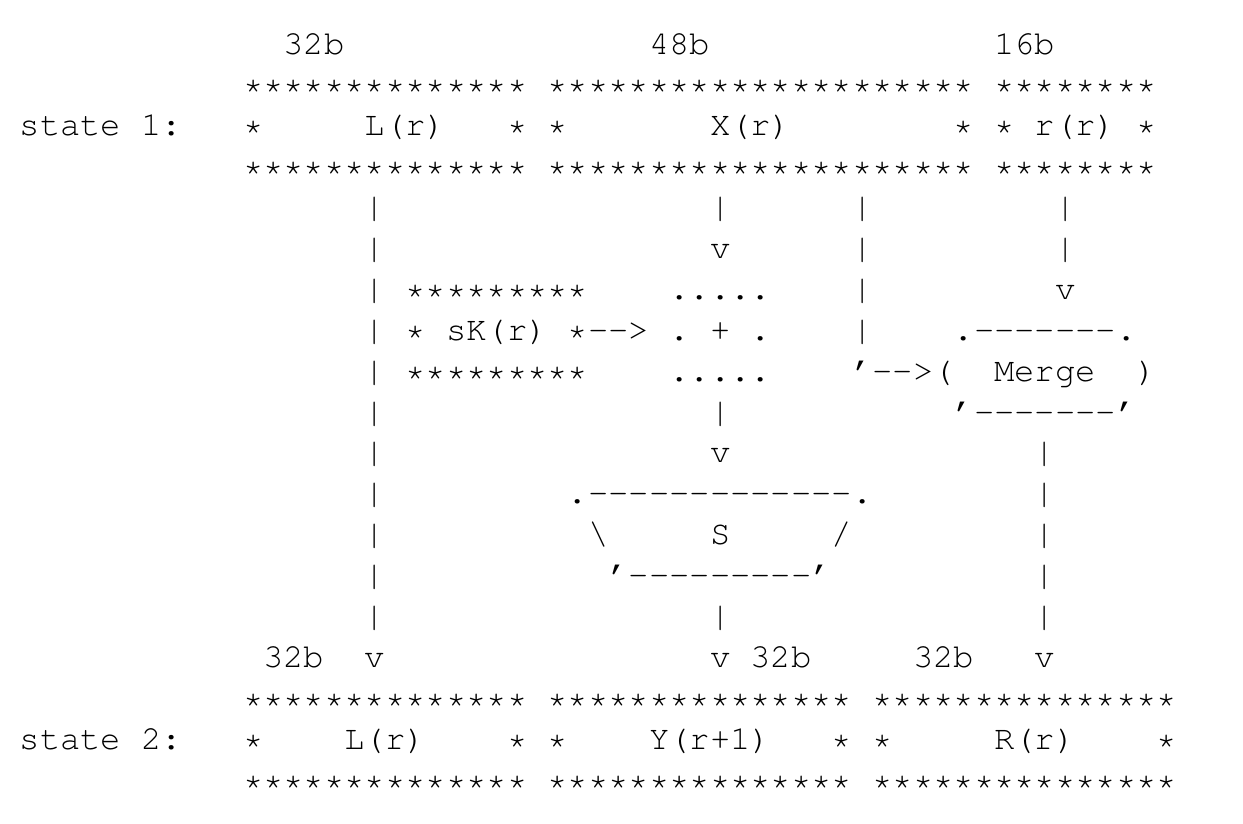
\includegraphics[scale=0.20]{images/etape_1_avant.png}

\end{figure}

\begin{figure}[h]
\centering
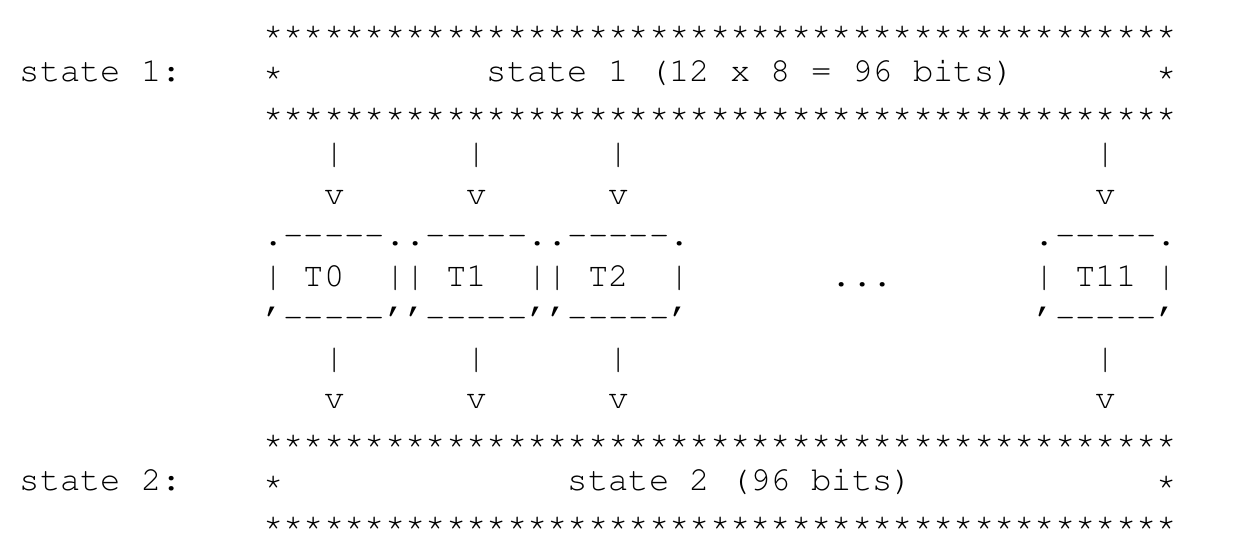
\includegraphics[scale=0.20]{images/etape_1_apres.png}
\end{figure}
\end{frame}


\begin{frame}{Décomposition de Matrice}
\begin{figure}[h]
\centering
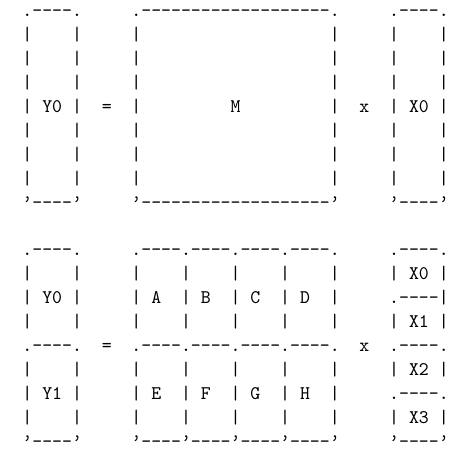
\includegraphics[scale=0.50]{images/decompo_matrice.png}
\caption{Décomposition de Matrice}
\label{fig:keygen}
\end{figure}
\end{frame}

\subsection{Input/Output Encoding}

\begin{frame}{Input / Output Encoding}
\begin{figure}[h]
\centering
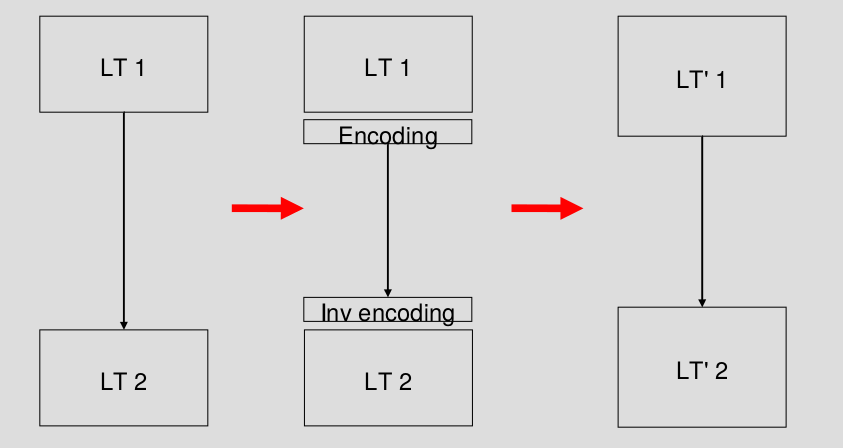
\includegraphics[scale=0.5]{images/encoding.png}
\caption{Encoding}
\label{fig:keygen}
\end{figure}
\end{frame}

\section{Concepts secondaires}

\subsection{Randomization}

\subsection{Mixing Bijection}

\subsection{Bypass}

\subsection{Combined Function Encoding}

\subsection{Split-Path Encoding}

\subsection{External Encoding}

\section{Conclusion}

\begin{frame}{Conclusion}
  
  \begin{itemize}
  \item Beaucoup d'effort pour d'autres solutions (API, clés publiques)
  \item Taille importante
  \item La non-connaissance des algorithmes est ``trop'' importante.
  \item Utilisé profesionnellement
  \end{itemize}

\end{frame}

\end{document}
